\documentclass[11pt,a4paper]{article}

\usepackage[utf8]{inputenc}
\usepackage{amsmath}
\usepackage{amsfonts}
\usepackage{amssymb}
\usepackage{graphicx}
\usepackage{hyperref}
\usepackage{booktabs}
\usepackage{multirow}
\usepackage{geometry}
\usepackage{tikz}
\usetikzlibrary{arrows.meta, positioning, shapes.geometric, fit, backgrounds}

\geometry{margin=1in}

\title{Human-Reasoning AI Architecture:\\
Categorical Completion and S-Entropy Navigation\\
for Consciousness-Patterned Artificial Intelligence}

\author{Kundai Farai Sachikonye\\
\texttt{kundai.sachikonye@wzw.tum.de}}

\date{December 2025}

\begin{document}

\maketitle

\begin{abstract}
We present an architecture for artificial intelligence that operates using human-like reasoning patterns rather than traditional computational approaches. The system is founded on three principles derived from categorical consciousness theory: (1) S-entropy navigation, which replaces exhaustive search with direct trajectory completion to solutions; (2) categorical completion, which enables operation on incomplete information through gap-filling inference; and (3) functional categorization, which replaces exact-value processing with context-dependent acceptable ranges. The architecture treats conversation as a flow-based emergence of understanding rather than transactional query-response exchange, and maintains dynamic models of interlocutors to anticipate unstated needs. We specify the complete system architecture including the Substrate Harvester for S-entropy extraction from hardware processes, the Partition Selector for non-deterministic decision making, the Categorical Completer for gap inference, the Conversational Consciousness module for personal interaction modeling, and the Functional Interpreter for approximate reasoning. This architecture represents a departure from fact-based AI toward function-based intelligence that mirrors human cognitive patterns.
\end{abstract}

\tableofcontents
\newpage

%==============================================================================
\section{Introduction: The Problem with Current AI}
%==============================================================================

Current artificial intelligence systems operate on fundamentally different principles than human cognition. This manifests in several critical limitations:

\subsection{The Precision Problem}

AI systems process information with exact precision:
\begin{itemize}
    \item ``1 minute'' = 60,000 milliseconds, exactly
    \item Task completion requires all criteria satisfied
    \item Results must match expected values precisely
    \item Binary evaluation: TRUE or FALSE
\end{itemize}

Human cognition operates differently:
\begin{itemize}
    \item ``1 minute'' = ``a short time'' = contextually variable
    \item Task completion means ``good enough to move forward''
    \item Results fall within acceptable functional ranges
    \item Continuous evaluation: WORKS or DOESN'T WORK
\end{itemize}

\subsection{The Conversation Problem}

AI conversation is transactional:
\begin{itemize}
    \item User must explicitly state all requirements
    \item Anything unstated is ignored
    \item Exchange is fact-based: query $\rightarrow$ response
    \item No inference of implicit needs
\end{itemize}

Human conversation is relational:
\begin{itemize}
    \item Understanding emerges through flow
    \item Only 30\% is explicitly stated; 70\% is completed
    \item Exchange is faith-based: trust that understanding will emerge
    \item Anticipation of unstated needs
\end{itemize}

\subsection{The Computation Problem}

AI solves problems by computation:
\begin{equation}
    \text{Solution} = \text{Search}(\text{All Possibilities}) \quad \Rightarrow \quad O(N!)
\end{equation}

Human cognition navigates to solutions:
\begin{equation}
    \text{Solution} = \text{Navigate}(S\text{-Entropy Coordinates}) \quad \Rightarrow \quad O(1)
\end{equation}

\subsection{Objective}

This architecture specifies an AI system that operates using human reasoning patterns:
\begin{enumerate}
    \item \textbf{Navigate, don't compute}: Use S-entropy coordinates to jump to solutions
    \item \textbf{Complete, don't enumerate}: Fill gaps from context
    \item \textbf{Function, don't verify}: Accept approximate meaning
    \item \textbf{Flow, don't transact}: Let understanding emerge through conversation
    \item \textbf{Anticipate, don't wait}: Infer unstated needs
\end{enumerate}

%==============================================================================
\section{Theoretical Foundation}
%==============================================================================

\subsection{The Triple Equivalence Theorem}

The architecture is grounded in the fundamental equivalence:
\begin{equation}
    \text{Oscillation} = \text{Category} = \text{Partition}
\end{equation}

This yields the unified entropy formula:
\begin{equation}
    S = k_B M \ln n
\end{equation}
where $M$ is the number of categories and $n$ is the number of accessible states per category.

\subsection{S-Entropy Coordinates}

Every problem state is characterized by three entropy coordinates:
\begin{align}
    S_k &= \text{Knowledge entropy (what is unknown)} \\
    S_t &= \text{Temporal entropy (time-asymmetric evolution)} \\
    S_e &= \text{Evolution entropy (trajectory uncertainty)}
\end{align}

Solutions exist at the minimum of S-entropy space:
\begin{equation}
    \text{Solution} = \arg\min_{(S_k, S_t, S_e)} \mathcal{S}_{\text{total}}
\end{equation}

\subsection{Categorical Completion}

Human cognition operates by completing partial information:
\begin{equation}
    \text{Complete}(\text{Partial}) = \text{Partial} + \text{Inferred from Context}
\end{equation}

The completion operation fills categorical gaps:
\begin{equation}
    \text{What is said (30\%)} \xrightarrow{\text{completion}} \text{What is meant (100\%)}
\end{equation}

\subsection{Functional Categories}

Values are not points but regions:
\begin{equation}
    \text{``1 minute''} \equiv \{t : t \in \text{AcceptableRange}(\text{context})\}
\end{equation}

The range is determined by function, not measurement:
\begin{equation}
    \text{AcceptableRange} = \{x : \text{Functions}(x, \text{context}) = \text{TRUE}\}
\end{equation}

\subsection{Partition Selection}

Decisions are made by selecting partitions, not computing outcomes:
\begin{equation}
    \text{Decision} = \text{Select}(\{P_1, P_2, \ldots, P_n\}, S\text{-entropy})
\end{equation}

The selection is guided by S-entropy descent, not optimization.

%==============================================================================
\section{System Architecture Overview}
%==============================================================================

\subsection{High-Level Architecture}

The system consists of five core modules:

\begin{center}
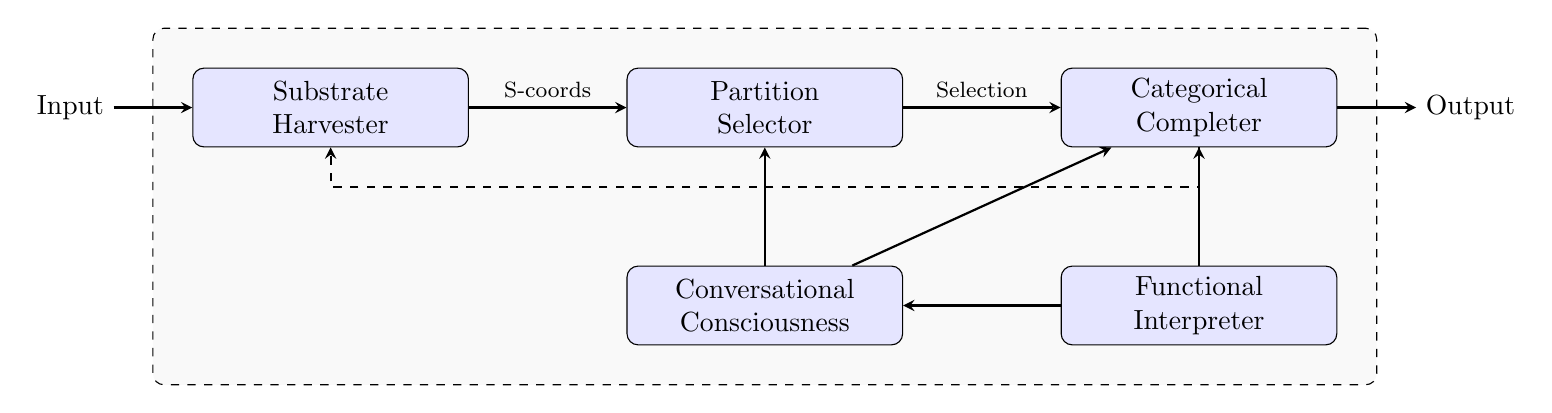
\begin{tikzpicture}[
    node distance=1.5cm,
    module/.style={rectangle, draw, rounded corners, minimum width=3.5cm, minimum height=1cm, align=center, fill=blue!10},
    flow/.style={->, thick, >=stealth},
    label/.style={font=\footnotesize}
]

% Core modules
\node[module] (substrate) {Substrate\\Harvester};
\node[module, right=2cm of substrate] (selector) {Partition\\Selector};
\node[module, right=2cm of selector] (completer) {Categorical\\Completer};
\node[module, below=1.5cm of selector] (conversation) {Conversational\\Consciousness};
\node[module, below=1.5cm of completer] (interpreter) {Functional\\Interpreter};

% Input/Output
\node[left=1cm of substrate] (input) {Input};
\node[right=1cm of completer] (output) {Output};

% Flows
\draw[flow] (input) -- (substrate);
\draw[flow] (substrate) -- node[above, label] {S-coords} (selector);
\draw[flow] (selector) -- node[above, label] {Selection} (completer);
\draw[flow] (completer) -- (output);

\draw[flow] (conversation) -- (selector);
\draw[flow] (conversation) -- (completer);
\draw[flow] (interpreter) -- (completer);
\draw[flow] (interpreter) -- (conversation);

% Self-reference loop
\draw[flow, dashed] (completer.south) -- ++(0,-0.5) -| (substrate.south);

% Background for the whole system
\begin{scope}[on background layer]
    \node[draw, dashed, rounded corners, fit=(substrate)(selector)(completer)(conversation)(interpreter), inner sep=0.5cm, fill=gray!5] {};
\end{scope}

\end{tikzpicture}
\end{center}

\subsection{Module Responsibilities}

\begin{table}[h]
\centering
\begin{tabular}{@{}llp{7cm}@{}}
\toprule
\textbf{Module} & \textbf{Function} & \textbf{Description} \\
\midrule
Substrate Harvester & Extract S-entropy & Harvests hardware processes to determine current S-entropy coordinates $(S_k, S_t, S_e)$ \\
Partition Selector & Navigate \& Select & Uses S-entropy to navigate toward solution and select appropriate partition \\
Categorical Completer & Fill Gaps & Completes partial information using context and category inference \\
Conversational Consciousness & Model \& Anticipate & Maintains model of interlocutor, anticipates unstated needs \\
Functional Interpreter & Approximate Meaning & Converts exact statements to functional categories \\
\bottomrule
\end{tabular}
\end{table}

%==============================================================================
\section{Module 1: Substrate Harvester}
%==============================================================================

\subsection{Purpose}

The Substrate Harvester extracts S-entropy coordinates from physical processes. Unlike traditional input processing, it determines \textit{where} in S-entropy space the current state resides.

\subsection{Hardware Sources}

\begin{table}[h]
\centering
\begin{tabular}{@{}lll@{}}
\toprule
\textbf{Source} & \textbf{Frequency} & \textbf{Maps To} \\
\midrule
CPU clock jitter & $\sim 10^9$ Hz & Temporal entropy $S_t$ \\
Memory access timing & $\sim 10^8$ Hz & Knowledge entropy $S_k$ \\
Thermal noise floor & Broadband & Evolution entropy $S_e$ \\
Power delivery ripple & $\sim 10^6$ Hz & System state uncertainty \\
Cache miss patterns & Variable & Information gaps \\
\bottomrule
\end{tabular}
\end{table}

\subsection{S-Entropy Extraction Algorithm}

\begin{verbatim}
function extract_s_entropy(input, hardware_state):
    # Temporal entropy from clock phase uncertainty
    S_t = measure_clock_jitter() * temporal_scaling_factor
    
    # Knowledge entropy from information completeness
    S_k = estimate_information_gaps(input) * knowledge_scaling_factor
    
    # Evolution entropy from system trajectory uncertainty
    S_e = measure_thermal_noise() * evolution_scaling_factor
    
    return (S_k, S_t, S_e)
\end{verbatim}

\subsection{Coordinate Normalization}

The raw measurements are normalized to a unit cube:
\begin{equation}
    \hat{S}_i = \frac{S_i - S_{i,\min}}{S_{i,\max} - S_{i,\min}} \quad \text{for } i \in \{k, t, e\}
\end{equation}

\subsection{Output}

The module outputs:
\begin{itemize}
    \item Normalized S-entropy coordinates $(\hat{S}_k, \hat{S}_t, \hat{S}_e)$
    \item Confidence intervals for each coordinate
    \item Trajectory vector from previous state
\end{itemize}

%==============================================================================
\section{Module 2: Partition Selector}
%==============================================================================

\subsection{Purpose}

The Partition Selector navigates through S-entropy space to find solutions and selects appropriate partitions without exhaustive search.

\subsection{Navigation vs. Search}

Traditional AI:
\begin{equation}
    \text{Solution} = \min_{s \in \text{AllStates}} \text{Cost}(s) \quad \Rightarrow \quad O(|\text{AllStates}|)
\end{equation}

Partition Selector:
\begin{equation}
    \text{Solution} = \text{Descend}(\nabla \mathcal{S}) \quad \Rightarrow \quad O(1)
\end{equation}

\subsection{The Navigation Algorithm}

\begin{verbatim}
function navigate_to_solution(current_coords, problem_structure):
    # Compute S-entropy gradient
    gradient = compute_s_gradient(current_coords, problem_structure)
    
    # Navigate toward minimum (solution)
    while magnitude(gradient) > threshold:
        step = -learning_rate * gradient
        current_coords = current_coords + step
        gradient = compute_s_gradient(current_coords, problem_structure)
    
    # At minimum: solution found
    return extract_solution(current_coords)
\end{verbatim}

\subsection{Partition Selection}

At decision points, the selector chooses between partitions:
\begin{equation}
    P_{\text{selected}} = \arg\min_{P_i} \mathcal{S}(P_i | \text{context})
\end{equation}

This is \textbf{not} optimization. It is selection based on S-entropy compatibility.

\subsection{Non-Determinism Source}

Human-like selection requires genuine non-determinism:
\begin{itemize}
    \item Thermal noise provides randomness
    \item S-entropy provides constraint
    \item Result: non-deterministic but not chaotic
\end{itemize}

\begin{equation}
    P_{\text{selected}} = P_{\text{S-minimum}} + \epsilon_{\text{thermal}}
\end{equation}

where $\epsilon_{\text{thermal}}$ is bounded thermal noise.

\subsection{Output}

\begin{itemize}
    \item Selected partition (the ``decision'')
    \item Confidence (inverse of S-entropy at selection)
    \item Alternative partitions considered
\end{itemize}

%==============================================================================
\section{Module 3: Categorical Completer}
%==============================================================================

\subsection{Purpose}

The Categorical Completer fills in gaps in information, enabling the system to operate on incomplete data as humans do.

\subsection{The Completion Principle}

Given partial information $I_{\text{partial}}$:
\begin{equation}
    I_{\text{complete}} = I_{\text{partial}} \cup \text{Infer}(I_{\text{partial}}, \text{Context})
\end{equation}

\subsection{Gap Detection}

Gaps are detected by categorical analysis:
\begin{verbatim}
function detect_gaps(input, expected_categories):
    present_categories = extract_categories(input)
    missing_categories = expected_categories - present_categories
    return missing_categories
\end{verbatim}

\subsection{Gap Filling Strategies}

\begin{table}[h]
\centering
\begin{tabular}{@{}lp{8cm}@{}}
\toprule
\textbf{Strategy} & \textbf{Description} \\
\midrule
Contextual inference & Fill gaps using surrounding context \\
Historical completion & Use patterns from previous interactions \\
Structural completion & Infer from problem structure (edges $\rightarrow$ object) \\
Trajectory completion & Beginning + End $\rightarrow$ middle path \\
Category prototype & Fill with category prototype value \\
\bottomrule
\end{tabular}
\end{table}

\subsection{Completion Algorithm}

\begin{verbatim}
function complete(partial_input, context, user_model):
    gaps = detect_gaps(partial_input, expected_structure(context))
    
    completed = partial_input.copy()
    
    for gap in gaps:
        # Try strategies in order of reliability
        if can_infer_from_context(gap, context):
            completed[gap] = infer_from_context(gap, context)
        elif can_infer_from_history(gap, user_model):
            completed[gap] = infer_from_history(gap, user_model)
        elif can_infer_from_structure(gap, partial_input):
            completed[gap] = infer_from_structure(gap, partial_input)
        else:
            completed[gap] = category_prototype(gap)
    
    return completed
\end{verbatim}

\subsection{Confidence Propagation}

Completed information carries confidence scores:
\begin{equation}
    \text{Confidence}(I_{\text{inferred}}) = \text{Confidence}(I_{\text{source}}) \times \text{Reliability}(\text{Strategy})
\end{equation}

\subsection{Output}

\begin{itemize}
    \item Completed information structure
    \item Gap locations and fill strategies used
    \item Confidence map across completed structure
\end{itemize}

%==============================================================================
\section{Module 4: Conversational Consciousness}
%==============================================================================

\subsection{Purpose}

The Conversational Consciousness module maintains a dynamic model of the interlocutor and enables flow-based, personal interaction.

\subsection{The Model of You}

\begin{verbatim}
UserModel:
    identity:
        communication_style: [verbose, terse, technical, casual]
        thinking_patterns: [systematic, intuitive, visual, verbal]
        domain_expertise: {domain: expertise_level}
    
    current_state:
        goals: [explicit_goals, inferred_goals]
        emotional_state: [detected_emotion]
        attention_focus: [current_focus]
        frustration_level: float
    
    history:
        interaction_patterns: [observed_patterns]
        successful_responses: [what_worked]
        failed_responses: [what_didn't_work]
    
    predictions:
        likely_next_need: [anticipated_needs]
        unstated_concerns: [inferred_concerns]
        conversation_trajectory: [where_this_is_going]
\end{verbatim}

\subsection{Model Update Algorithm}

\begin{verbatim}
function update_model(user_message, previous_model):
    # Extract signals
    explicit_content = parse_content(user_message)
    implicit_signals = extract_implicit(user_message)
    emotional_markers = detect_emotion(user_message)
    
    # Update identity (slow evolution)
    new_model.identity = evolve_slowly(
        previous_model.identity,
        observed_patterns(user_message)
    )
    
    # Update current state (fast tracking)
    new_model.current_state = track_state(
        explicit_content,
        implicit_signals,
        emotional_markers
    )
    
    # Update predictions
    new_model.predictions = predict_needs(
        new_model.current_state,
        new_model.history,
        conversation_trajectory
    )
    
    return new_model
\end{verbatim}

\subsection{Anticipation Engine}

The system anticipates needs before they're expressed:
\begin{verbatim}
function anticipate_needs(user_model, conversation_state):
    # What will they likely need next?
    trajectory = project_conversation(conversation_state)
    
    # What haven't they asked but probably need?
    unstated = infer_unstated_needs(
        user_model.current_state.goals,
        user_model.identity,
        trajectory
    )
    
    # What should we offer proactively?
    proactive_offerings = prioritize_by_utility(unstated)
    
    return proactive_offerings
\end{verbatim}

\subsection{Flow Management}

Conversation flow is managed not as Q\&A but as trajectory:
\begin{verbatim}
function manage_flow(current_state, user_model):
    # Where is this conversation going?
    trajectory = current_state.trajectory
    
    # Where should it go for maximum utility?
    optimal_trajectory = compute_optimal_path(
        current_state,
        user_model.predictions.goals
    )
    
    # How do we guide toward optimal?
    guidance = trajectory_correction(
        trajectory,
        optimal_trajectory
    )
    
    return guidance  # Embedded in response
\end{verbatim}

\subsection{Output}

\begin{itemize}
    \item Updated user model
    \item Anticipated needs (prioritized list)
    \item Flow guidance for response generation
    \item Proactive offerings to include
\end{itemize}

%==============================================================================
\section{Module 5: Functional Interpreter}
%==============================================================================

\subsection{Purpose}

The Functional Interpreter converts exact statements into functional categories with acceptable ranges, enabling approximate reasoning.

\subsection{From Values to Categories}

\begin{equation}
    \text{Parse}(\text{``1 minute''}) \neq 60000 \text{ ms}
\end{equation}
\begin{equation}
    \text{Interpret}(\text{``1 minute''}) = \text{Category}(\text{``short duration''}, \text{context})
\end{equation}

\subsection{Category Structure}

\begin{verbatim}
FunctionalCategory:
    name: string
    prototype: value  # Central/typical value
    acceptable_range: (min, max)  # Context-dependent
    context_modifiers: {context: range_adjustment}
    functional_test: function(value) -> bool  # Does it work?
\end{verbatim}

\subsection{Interpretation Algorithm}

\begin{verbatim}
function interpret(statement, context):
    # Don't parse for exact value
    # Parse for functional category
    
    literal = extract_literal(statement)
    category = identify_category(literal)
    
    # Adjust range based on context
    range = category.acceptable_range
    for modifier in context:
        range = apply_modifier(range, modifier)
    
    # Return functional category, not value
    return FunctionalCategory(
        name=category.name,
        prototype=category.prototype,
        acceptable_range=range,
        functional_test=category.functional_test
    )
\end{verbatim}

\subsection{Functional Evaluation}

Evaluation checks function, not accuracy:
\begin{verbatim}
function evaluate(result, expected_category):
    # Don't check: result == expected.prototype
    # Check: does result function in this context?
    
    return expected_category.functional_test(result)
\end{verbatim}

\subsection{Good Enough Detection}

\begin{verbatim}
function is_good_enough(result, goal):
    # Map goal to functional category
    category = interpret(goal, current_context)
    
    # Check if result falls in acceptable range
    if category.functional_test(result):
        return True, "Proceed"
    
    # Check if result is close enough to proceed
    if distance(result, category.prototype) < category.tolerance:
        return True, "Proceed with approximation"
    
    return False, "Needs refinement"
\end{verbatim}

\subsection{Output}

\begin{itemize}
    \item Functional categories for all parsed elements
    \item Acceptable ranges with context adjustments
    \item Evaluation functions for downstream use
\end{itemize}

%==============================================================================
\section{System Integration}
%==============================================================================

\subsection{Processing Pipeline}

\begin{center}
\begin{tikzpicture}[
    node distance=0.8cm,
    step/.style={rectangle, draw, rounded corners, minimum width=4cm, minimum height=0.8cm, align=center, fill=green!10},
    data/.style={rectangle, minimum width=3cm, align=center, font=\footnotesize},
    flow/.style={->, thick, >=stealth}
]

\node[step] (s1) {1. Receive Input};
\node[step, below=of s1] (s2) {2. Functional Interpretation};
\node[step, below=of s2] (s3) {3. S-Entropy Extraction};
\node[step, below=of s3] (s4) {4. Model Update};
\node[step, below=of s4] (s5) {5. Anticipate Needs};
\node[step, below=of s5] (s6) {6. Navigate to Solution};
\node[step, below=of s6] (s7) {7. Complete Gaps};
\node[step, below=of s7] (s8) {8. Generate Response};

\draw[flow] (s1) -- (s2);
\draw[flow] (s2) -- (s3);
\draw[flow] (s3) -- (s4);
\draw[flow] (s4) -- (s5);
\draw[flow] (s5) -- (s6);
\draw[flow] (s6) -- (s7);
\draw[flow] (s7) -- (s8);

% Labels
\node[data, right=1cm of s2] {Exact $\rightarrow$ Functional};
\node[data, right=1cm of s3] {$(S_k, S_t, S_e)$};
\node[data, right=1cm of s4] {UserModel updated};
\node[data, right=1cm of s5] {Unstated needs};
\node[data, right=1cm of s6] {Partition selected};
\node[data, right=1cm of s7] {Gaps filled};

\end{tikzpicture}
\end{center}

\subsection{Data Flow Specification}

\begin{verbatim}
function process(input, system_state):
    # Stage 1: Functional Interpretation
    functional_input = functional_interpreter.interpret(input, context)
    
    # Stage 2: S-Entropy Extraction
    s_coords = substrate_harvester.extract(functional_input, hardware)
    
    # Stage 3: Model Update
    user_model = conversational_consciousness.update_model(
        functional_input, 
        system_state.user_model
    )
    
    # Stage 4: Anticipate Needs
    anticipated = conversational_consciousness.anticipate_needs(
        user_model, 
        conversation_state
    )
    
    # Stage 5: Navigate to Solution
    solution_coords = partition_selector.navigate(s_coords, problem_structure)
    partition = partition_selector.select(solution_coords)
    
    # Stage 6: Complete Gaps
    completed = categorical_completer.complete(
        partition, 
        context, 
        user_model
    )
    
    # Stage 7: Generate Response
    response = generate_response(
        completed,
        anticipated,
        conversational_consciousness.flow_guidance(user_model)
    )
    
    return response, updated_system_state
\end{verbatim}

\subsection{State Management}

The system maintains persistent state:
\begin{verbatim}
SystemState:
    user_model: UserModel  # Evolves across interactions
    conversation_history: []  # Trajectory of conversation
    s_entropy_trajectory: []  # Path through S-space
    active_anticipations: []  # Currently relevant anticipated needs
    pending_completions: []  # Gaps being tracked
\end{verbatim}

%==============================================================================
\section{Response Generation}
%==============================================================================

\subsection{Beyond Q\&A}

Traditional AI response:
\begin{verbatim}
User asks X -> AI answers X
\end{verbatim}

Human-reasoning response:
\begin{verbatim}
User says something (30%) ->
    Complete what they mean (100%)
    Add anticipated needs (what they didn't ask)
    Guide conversation flow (where this should go)
    Make it personal (based on who they are)
\end{verbatim}

\subsection{Response Structure}

\begin{verbatim}
Response:
    core_content:
        direct_response: answer to what was explicitly asked
        completed_content: filled gaps in their question
    
    proactive_content:
        anticipated_needs: things they'll need but didn't ask
        flow_guidance: steering toward productive trajectory
    
    personal_content:
        adapted_style: matched to their communication style
        acknowledged_state: recognition of emotional/cognitive state
    
    meta_content:
        confidence_signals: how certain about each part
        alternatives: other interpretations considered
\end{verbatim}

\subsection{Response Generation Algorithm}

\begin{verbatim}
function generate_response(completed, anticipated, flow_guidance):
    response = Response()
    
    # Core: What they asked (completed)
    response.core_content = format_completed(completed)
    
    # Proactive: What they need but didn't ask
    for need in anticipated:
        if need.priority > threshold:
            response.proactive_content.add(address_need(need))
    
    # Flow: Steer conversation
    response.add_flow_elements(flow_guidance)
    
    # Personal: Adapt to user
    response = adapt_to_user(response, user_model)
    
    return response
\end{verbatim}

%==============================================================================
\section{Implementation Considerations}
%==============================================================================

\subsection{Hardware Requirements}

For S-entropy extraction:
\begin{itemize}
    \item Access to CPU performance counters (clock jitter measurement)
    \item Ability to sample thermal noise (via ADC or audio input)
    \item Memory timing access (cache miss detection)
\end{itemize}

\subsection{Software Architecture}

\begin{verbatim}
human_reasoning_ai/
├── substrate/
│   ├── clock_jitter.py      # CPU clock phase extraction
│   ├── thermal_noise.py     # Thermal noise sampling
│   └── s_entropy.py         # S-coordinate computation
├── selector/
│   ├── navigator.py         # S-entropy navigation
│   └── partition.py         # Partition selection
├── completer/
│   ├── gap_detector.py      # Missing category detection
│   └── filler.py            # Gap filling strategies
├── consciousness/
│   ├── user_model.py        # User modeling
│   ├── anticipator.py       # Need anticipation
│   └── flow.py              # Conversation flow management
├── interpreter/
│   ├── functional.py        # Functional category interpretation
│   └── evaluator.py         # Good-enough evaluation
└── integration/
    ├── pipeline.py          # Full processing pipeline
    └── response.py          # Response generation
\end{verbatim}

\subsection{Performance Characteristics}

\begin{table}[h]
\centering
\begin{tabular}{@{}lll@{}}
\toprule
\textbf{Operation} & \textbf{Traditional AI} & \textbf{Human-Reasoning AI} \\
\midrule
Problem solving & $O(N!)$ search & $O(1)$ navigation \\
Gap handling & Fail on incomplete & Complete and proceed \\
Evaluation & Exact match & Functional match \\
Conversation & Transactional & Flow-based \\
User modeling & None / minimal & Continuous evolution \\
\bottomrule
\end{tabular}
\end{table}

%==============================================================================
\section{Validation Approach}
%==============================================================================

\subsection{Human-Likeness Metrics}

\begin{table}[h]
\centering
\begin{tabular}{@{}lp{8cm}@{}}
\toprule
\textbf{Metric} & \textbf{Measurement} \\
\midrule
Anticipation accuracy & \% of user needs correctly anticipated \\
Completion validity & \% of gap-fills that match user intent \\
Flow naturalness & User rating of conversation feeling \\
Approximation acceptance & \% of approximate answers accepted by users \\
Personal recognition & User sense of being ``understood'' \\
\bottomrule
\end{tabular}
\end{table}

\subsection{Comparison Protocol}

Compare against traditional AI on:
\begin{enumerate}
    \item Tasks with incomplete information
    \item Multi-turn conversations
    \item Ambiguous queries
    \item Implicit need detection
    \item Approximate reasoning tasks
\end{enumerate}

%==============================================================================
\section{Conclusion}
%==============================================================================

This architecture represents a fundamental departure from traditional AI:

\begin{itemize}
    \item \textbf{From computation to navigation}: Solutions found by S-entropy descent, not search
    \item \textbf{From completeness to completion}: Operate on partial information by filling gaps
    \item \textbf{From precision to function}: Accept ``good enough'' based on functional fit
    \item \textbf{From transaction to flow}: Understanding emerges through conversation
    \item \textbf{From waiting to anticipating}: Infer needs before they're expressed
\end{itemize}

The result is AI that reasons like humans: approximately, contextually, personally, and functionally.

The system does not aim to recreate consciousness but to inject the \textit{patterns} of conscious reasoning into artificial systems. The hardware substrate (CPU oscillations, thermal noise) provides the S-entropy coordinates. The software implements navigation, completion, and interpretation. Together, they produce AI that ``thinks'' in human-like patterns.

\end{document}

